\documentclass{standalone}
\usepackage{tikz}
\usetikzlibrary{patterns, positioning}
\usepackage[sfdefault]{ClearSans} %% option 'sfdefault' activates Clear Sans as the default text font
\usepackage[T1]{fontenc}

\begin{document}
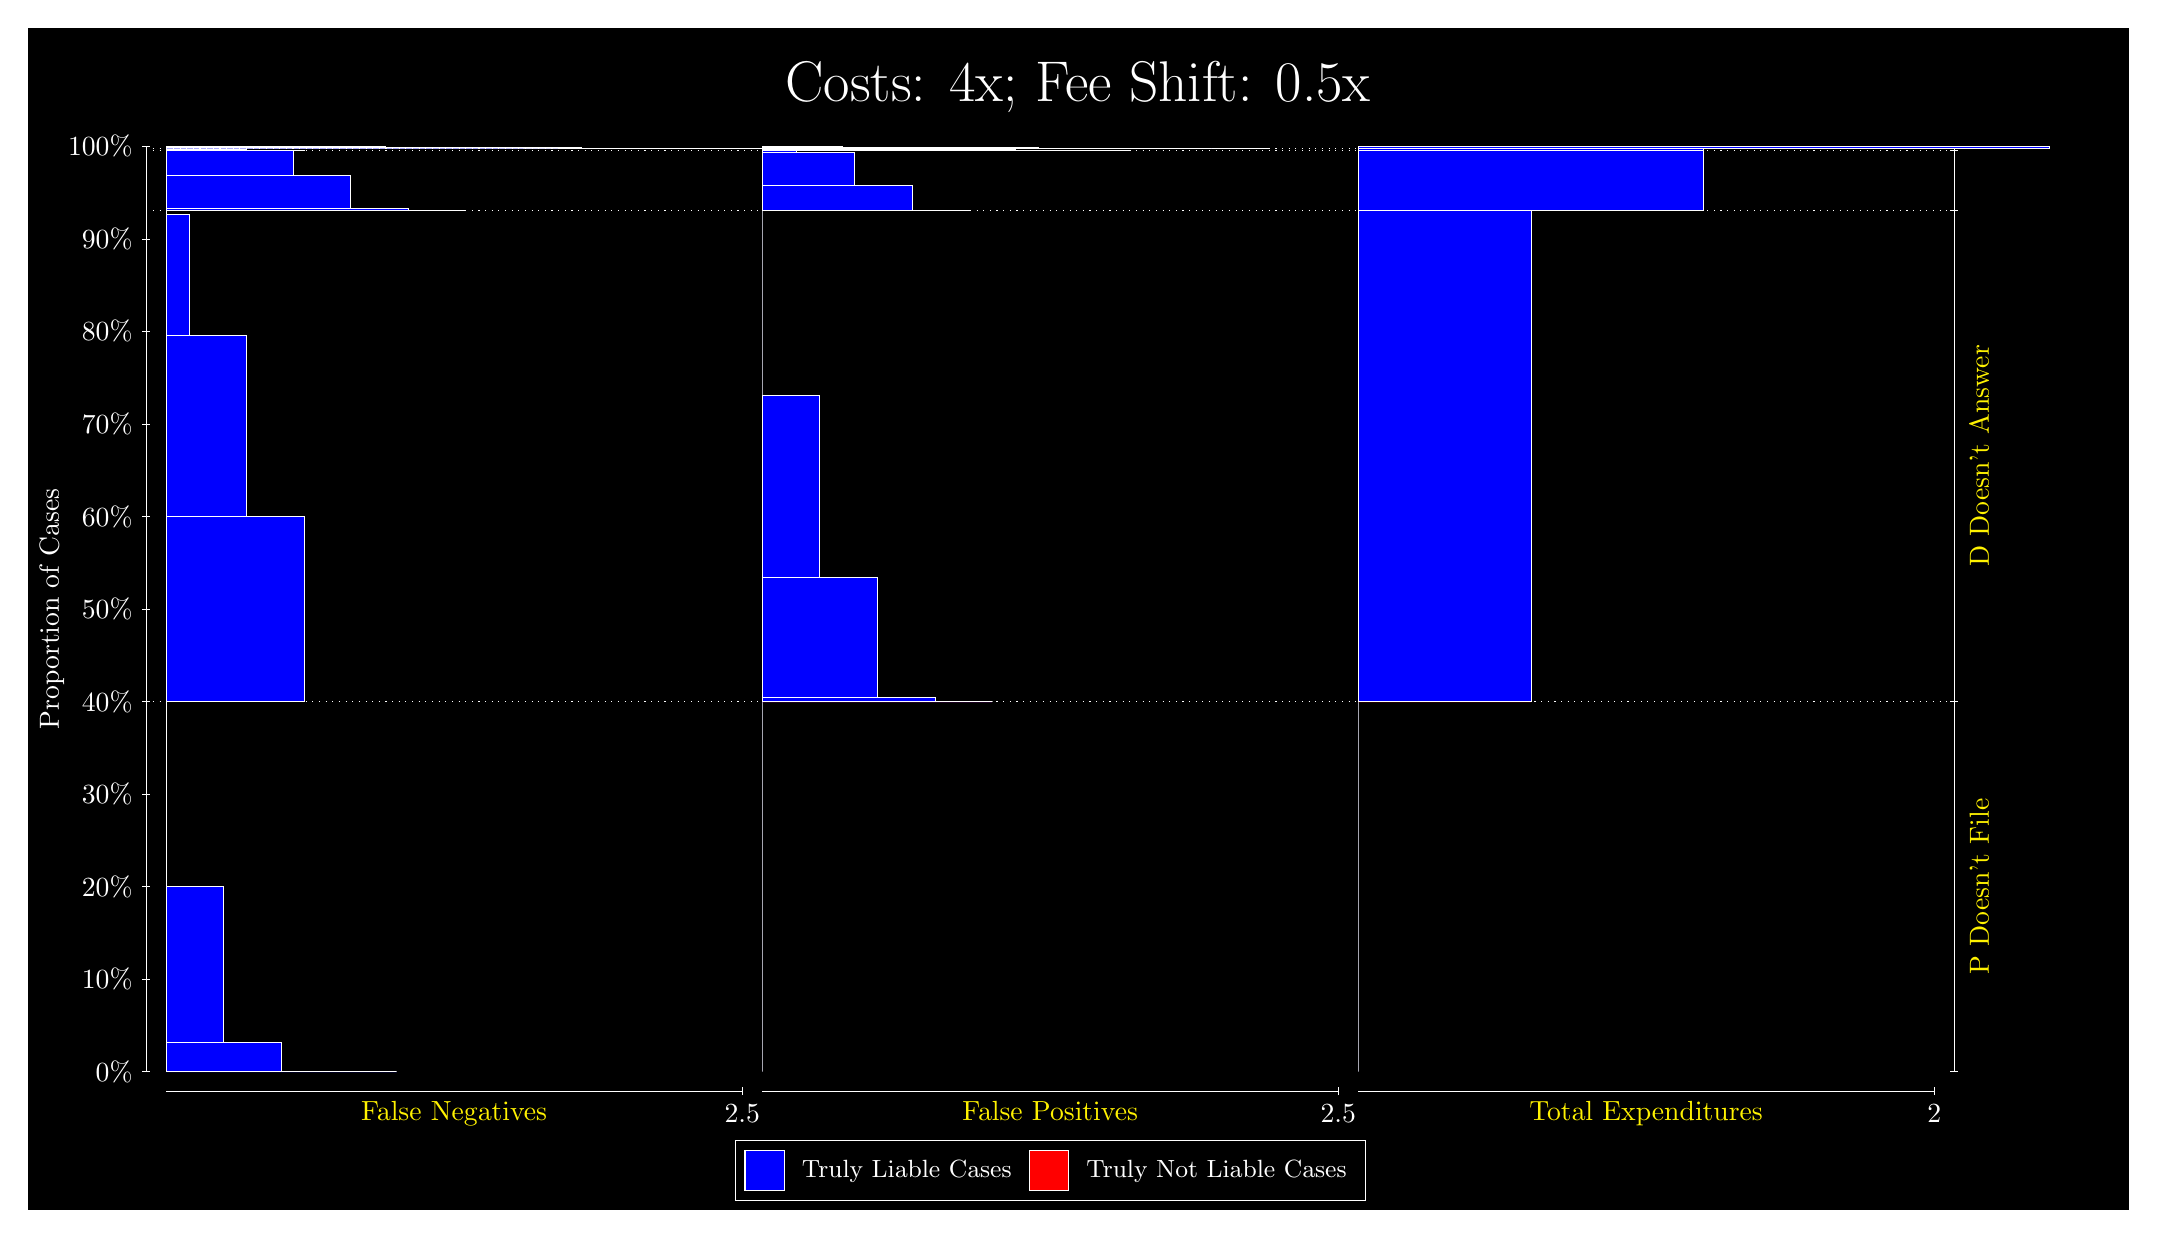
\begin{tikzpicture}
\draw[fill=black] (0,0) rectangle (26.667,15);
\draw[text=white] (0,13.5) rectangle (26.667,15) node[midway] {\huge Costs: 4x; Fee Shift: 0.5x};
\draw[white, very thin] (1.5,1.75) -- (1.5,13.5);
\node[rotate=90, text=white, anchor=center] at (0.3, 7.625) {Proportion of Cases};
\draw[white, very thin] (1.45,1.75) -- (1.55,1.75);
\node[text=white, anchor=east] at (1.45, 1.75) {0\%};
\draw[white, very thin] (1.45,2.925) -- (1.55,2.925);
\node[text=white, anchor=east] at (1.45, 2.925) {10\%};
\draw[white, very thin] (1.45,4.1) -- (1.55,4.1);
\node[text=white, anchor=east] at (1.45, 4.1) {20\%};
\draw[white, very thin] (1.45,5.275) -- (1.55,5.275);
\node[text=white, anchor=east] at (1.45, 5.275) {30\%};
\draw[white, very thin] (1.45,6.45) -- (1.55,6.45);
\node[text=white, anchor=east] at (1.45, 6.45) {40\%};
\draw[white, very thin] (1.45,7.625) -- (1.55,7.625);
\node[text=white, anchor=east] at (1.45, 7.625) {50\%};
\draw[white, very thin] (1.45,8.8) -- (1.55,8.8);
\node[text=white, anchor=east] at (1.45, 8.8) {60\%};
\draw[white, very thin] (1.45,9.975) -- (1.55,9.975);
\node[text=white, anchor=east] at (1.45, 9.975) {70\%};
\draw[white, very thin] (1.45,11.15) -- (1.55,11.15);
\node[text=white, anchor=east] at (1.45, 11.15) {80\%};
\draw[white, very thin] (1.45,12.325) -- (1.55,12.325);
\node[text=white, anchor=east] at (1.45, 12.325) {90\%};
\draw[white, very thin] (1.45,13.5) -- (1.55,13.5);
\node[text=white, anchor=east] at (1.45, 13.5) {100\%};

\draw[white, very thin] (24.457,1.75) -- (24.457,13.5);
\draw[white, very thin] (24.407,1.75) -- (24.507,1.75);
\node[anchor=west] at (24.407, 1.75) {};
\draw[white, very thin] (24.407,6.4489) -- (24.507,6.4489);
\node[anchor=west] at (24.407, 6.4489) {};
\draw[white, very thin] (24.407,12.686) -- (24.507,12.686);
\node[anchor=west] at (24.407, 12.686) {};
\draw[white, very thin] (24.407,13.449) -- (24.507,13.449);
\node[anchor=west] at (24.407, 13.449) {};
\draw[white, very thin] (24.407,13.475) -- (24.507,13.475);
\node[anchor=west] at (24.407, 13.475) {};
\draw[white, very thin] (24.407,13.5) -- (24.507,13.5);
\node[anchor=west] at (24.407, 13.5) {};

\draw[white, very thin, fill=blue] (1.75,1.75) rectangle (4.6775,1.75);
\draw[white, very thin, fill=blue] (1.75,1.75) rectangle (3.9457,1.7532);
\draw[white, very thin, fill=blue] (1.75,1.7532) rectangle (3.2138,2.126);
\draw[white, very thin, fill=blue] (1.75,2.126) rectangle (2.4819,4.1027);
\draw[white, very thin, fill=red] (1.75,4.1027) rectangle (1.75,4.1027);
\draw[white, very thin, fill=blue] (1.75,4.1027) rectangle (1.75,6.4489);
\draw[white, very thin, fill=blue] (1.75,6.4489) rectangle (3.5065,8.7985);
\draw[white, very thin, fill=blue] (1.75,8.7985) rectangle (2.7746,11.105);
\draw[white, very thin, fill=blue] (1.75,11.105) rectangle (2.0428,12.633);
\draw[white, very thin, fill=red] (1.75,12.633) rectangle (1.75,12.633);
\draw[white, very thin, fill=blue] (1.75,12.633) rectangle (1.75,12.686);
\draw[white, very thin, fill=blue] (1.75,12.686) rectangle (5.5558,12.686);
\draw[white, very thin, fill=blue] (1.75,12.686) rectangle (4.8239,12.71);
\draw[white, very thin, fill=blue] (1.75,12.71) rectangle (4.092,13.127);
\draw[white, very thin, fill=blue] (1.75,13.127) rectangle (3.3602,13.446);
\draw[white, very thin, fill=blue] (1.75,13.446) rectangle (2.6283,13.449);
\draw[white, very thin, fill=red] (1.75,13.449) rectangle (1.75,13.449);
\draw[white, very thin, fill=blue] (1.75,13.449) rectangle (3.5065,13.45);
\draw[white, very thin, fill=blue] (1.75,13.45) rectangle (2.7746,13.465);
\draw[white, very thin, fill=blue] (1.75,13.465) rectangle (2.0428,13.475);
\draw[white, very thin, fill=red] (1.75,13.475) rectangle (1.75,13.475);
\draw[white, very thin, fill=blue] (1.75,13.475) rectangle (1.75,13.475);
\draw[white, very thin, fill=blue] (1.75,13.475) rectangle (9.9471,13.475);
\draw[white, very thin, fill=blue] (1.75,13.475) rectangle (9.2152,13.475);
\draw[white, very thin, fill=blue] (1.75,13.475) rectangle (8.4834,13.476);
\draw[white, very thin, fill=blue] (1.75,13.476) rectangle (7.7515,13.481);
\draw[white, very thin, fill=blue] (1.75,13.481) rectangle (7.0196,13.482);
\draw[white, very thin, fill=blue] (1.75,13.482) rectangle (6.7268,13.482);
\draw[white, very thin, fill=blue] (1.75,13.482) rectangle (6.2877,13.482);
\draw[white, very thin, fill=blue] (1.75,13.482) rectangle (5.9949,13.482);
\draw[white, very thin, fill=blue] (1.75,13.482) rectangle (5.2631,13.494);
\draw[white, very thin, fill=blue] (1.75,13.494) rectangle (4.5312,13.499);
\draw[white, very thin, fill=blue] (1.75,13.499) rectangle (3.7993,13.5);
\draw[white, very thin, fill=blue] (1.75,13.5) rectangle (3.0674,13.5);
\draw[white, very thin, fill=blue] (1.75,13.5) rectangle (2.3355,13.5);
\draw[white, very thin, fill=red] (1.75,13.5) rectangle (1.75,13.5);
\draw[white, very thin, fill=red] (9.3189,1.75) rectangle (9.3189,1.75);
\draw[white, very thin, fill=blue] (9.3189,1.75) rectangle (9.3189,6.4489);
\draw[white, very thin, fill=red] (9.3189,6.4489) rectangle (12.246,6.4489);
\draw[white, very thin, fill=blue] (9.3189,6.4489) rectangle (12.246,6.4489);
\draw[white, very thin, fill=blue] (9.3189,6.4489) rectangle (11.515,6.5024);
\draw[white, very thin, fill=blue] (9.3189,6.5024) rectangle (10.783,8.0303);
\draw[white, very thin, fill=blue] (9.3189,8.0303) rectangle (10.051,10.337);
\draw[white, very thin, fill=blue] (9.3189,10.337) rectangle (9.3189,12.686);
\draw[white, very thin, fill=red] (9.3189,12.686) rectangle (11.954,12.686);
\draw[white, very thin, fill=blue] (9.3189,12.686) rectangle (11.954,12.69);
\draw[white, very thin, fill=blue] (9.3189,12.69) rectangle (11.222,13.009);
\draw[white, very thin, fill=blue] (9.3189,13.009) rectangle (10.49,13.426);
\draw[white, very thin, fill=blue] (9.3189,13.426) rectangle (9.758,13.449);
\draw[white, very thin, fill=blue] (9.3189,13.449) rectangle (9.3189,13.449);
\draw[white, very thin, fill=red] (9.3189,13.449) rectangle (14.003,13.449);
\draw[white, very thin, fill=blue] (9.3189,13.449) rectangle (14.003,13.449);
\draw[white, very thin, fill=blue] (9.3189,13.449) rectangle (13.271,13.45);
\draw[white, very thin, fill=blue] (9.3189,13.45) rectangle (12.539,13.459);
\draw[white, very thin, fill=blue] (9.3189,13.459) rectangle (11.807,13.475);
\draw[white, very thin, fill=blue] (9.3189,13.475) rectangle (11.075,13.475);
\draw[white, very thin, fill=red] (9.3189,13.475) rectangle (15.759,13.475);
\draw[white, very thin, fill=blue] (9.3189,13.475) rectangle (15.759,13.475);
\draw[white, very thin, fill=blue] (9.3189,13.475) rectangle (15.028,13.475);
\draw[white, very thin, fill=red] (9.3189,13.475) rectangle (15.028,13.475);
\draw[white, very thin, fill=blue] (9.3189,13.475) rectangle (15.028,13.475);
\draw[white, very thin, fill=blue] (9.3189,13.475) rectangle (14.296,13.476);
\draw[white, very thin, fill=red] (9.3189,13.476) rectangle (14.296,13.476);
\draw[white, very thin, fill=blue] (9.3189,13.476) rectangle (14.296,13.476);
\draw[white, very thin, fill=blue] (9.3189,13.476) rectangle (13.564,13.476);
\draw[white, very thin, fill=blue] (9.3189,13.476) rectangle (13.564,13.481);
\draw[white, very thin, fill=blue] (9.3189,13.481) rectangle (12.832,13.481);
\draw[white, very thin, fill=blue] (9.3189,13.481) rectangle (12.832,13.493);
\draw[white, very thin, fill=blue] (9.3189,13.493) rectangle (12.1,13.494);
\draw[white, very thin, fill=red] (9.3189,13.494) rectangle (11.807,13.494);
\draw[white, very thin, fill=blue] (9.3189,13.494) rectangle (11.807,13.494);
\draw[white, very thin, fill=blue] (9.3189,13.494) rectangle (11.368,13.494);
\draw[white, very thin, fill=red] (9.3189,13.494) rectangle (11.075,13.494);
\draw[white, very thin, fill=blue] (9.3189,13.494) rectangle (11.075,13.494);
\draw[white, very thin, fill=blue] (9.3189,13.494) rectangle (10.344,13.499);
\draw[white, very thin, fill=blue] (9.3189,13.499) rectangle (9.6116,13.5);
\draw[white, very thin, fill=blue] (9.3189,13.5) rectangle (9.3189,13.5);
\draw[white, very thin, fill=red] (16.888,1.75) rectangle (16.888,1.75);
\draw[white, very thin, fill=blue] (16.888,1.75) rectangle (16.888,6.4489);
\draw[white, very thin, fill=red] (16.888,6.4489) rectangle (19.083,6.4489);
\draw[white, very thin, fill=blue] (16.888,6.4489) rectangle (19.083,12.686);
\draw[white, very thin, fill=red] (16.888,12.686) rectangle (21.279,12.686);
\draw[white, very thin, fill=blue] (16.888,12.686) rectangle (21.279,13.449);
\draw[white, very thin, fill=red] (16.888,13.449) rectangle (21.279,13.449);
\draw[white, very thin, fill=blue] (16.888,13.449) rectangle (21.279,13.475);
\draw[white, very thin, fill=red] (16.888,13.475) rectangle (25.67,13.475);
\draw[white, very thin, fill=blue] (16.888,13.475) rectangle (25.67,13.476);
\draw[white, very thin, fill=red] (16.888,13.476) rectangle (25.67,13.476);
\draw[white, very thin, fill=blue] (16.888,13.476) rectangle (25.67,13.5);
\draw[white, dotted] (1.5,6.4489) -- (24.457,6.4489);
\draw[white, dotted] (1.5,12.686) -- (24.457,12.686);
\draw[white, dotted] (1.5,13.449) -- (24.457,13.449);
\draw[white, dotted] (1.5,13.475) -- (24.457,13.475);
\draw[white, very thin] (1.75,1.5) -- (9.0689,1.5);
\node[text=yellow, anchor=north] at (5.4094, 1.5) {False Negatives};
\draw[white, very thin] (9.0689,1.45) -- (9.0689,1.55);
\node[text=white, anchor=north] at (9.0689, 1.45) {2.5};

\draw[white, very thin] (9.3189,1.5) -- (16.638,1.5);
\node[text=yellow, anchor=north] at (12.978, 1.5) {False Positives};
\draw[white, very thin] (16.638,1.45) -- (16.638,1.55);
\node[text=white, anchor=north] at (16.638, 1.45) {2.5};

\draw[white, very thin] (16.888,1.5) -- (24.207,1.5);
\node[text=yellow, anchor=north] at (20.547, 1.5) {Total Expenditures};
\draw[white, very thin] (24.207,1.45) -- (24.207,1.55);
\node[text=white, anchor=north] at (24.207, 1.45) {2};

\node[text=yellow, centered, rotate=90] at (24.777, 4.0995) {P Doesn't File};
\node[text=yellow, centered, rotate=90] at (24.777, 9.5677) {D Doesn't Answer};




\draw (12.978300999999998,1.5) node[draw=none] (baseCoordinate) {};
\begin{scope}[align=center]
        \matrix[scale=0.5, draw=white, below=0.5cm of baseCoordinate, nodes={draw}, column sep=0.1cm]{
            \node[rectangle, draw, minimum width=0.5cm, minimum height=0.5cm, fill=blue] {}; &
            \node[draw=none, font=\small, text=white] (B) {Truly Liable Cases}; &
            \node[rectangle, draw, minimum width=0.5cm, minimum height=0.5cm, fill=red] {}; &
            \node[draw=none, font=\small, text=white] (B) {Truly Not Liable Cases}; \\
            };
\end{scope}

\end{tikzpicture}
\end{document}